\documentclass[a4paper,12pt]{article}
\usepackage[top=2cm,bottom=2cm,left=2cm,right=2cm]{geometry}
\usepackage[italian]{babel}
\usepackage{datetime}
\usepackage[utf8]{inputenc}
\usepackage{multicol}
\usepackage{textcomp}
\usepackage{amsmath}
\usepackage{gensymb}
\usepackage{graphicx}
\newcommand{\sen}{\textrm{sen}}
\newcommand{\tg}{\textrm{tg}}
\newcommand{\esempio}{\textbf{\textit{\large{Esempio: }}}}
\title{Fisica - Triennio}
\renewcommand{\arraystretch}{1.5}
\begin{document}
\maketitle
\section{I vettori}
\subsection{Forma cartesiana e forma polare}
\subsection{Somma di vettori}
\subsubsection{Metodo grafico}
\subsubsection{Metodo analitico}
\subsection{Differenza di vettori}
\subsubsection{Metodo grafico}
\subsubsection{Metodo analitico}
\subsection{Prodotto o divisione di un vettore per un numero}
\subsubsection{Metodo grafico}
\subsubsection{Metodo analitico}
\subsection{Vettori cinematici}
\subsubsection{Vettore posizione}
\subsubsection{Vettore spostamento}
\subsubsection{Vettore velocità media}
\subsubsection{Vettore velocità istantanea}
\subsection{I versori}
\par Sono da copiare dall'unità due prima della composizione di moti
\section{I moti}
\subsection{Moto rettilineo uniforme}
\subsection{Moto rettilineo uniformemente accelerato}
\subsection{Moto armonico}
\subsubsection{Analisi di moto armonico mediante TI-92+CBR}
\subsubsection{Equazioni orarie del moto armonico}
\subsection{Moto circolare}
\subsubsection{Lunghezza dell'arco di circonferenza}
\subsubsection{Equazione della circonferenza in coordinate cartesiane}
\subsubsection{Definizione di moto circolare uniforme}
\subsubsection{Periodo e frequenza nel moto circolare uniforme}
\subsubsection{Vettore velocità lineare}
\subsubsection{Velocità angolare}
\subsubsection{Accelerazione nel moto circolare uniforme}
\subsubsection{Equazioni lineari del moto circolare uniforme}
\subsubsection{Equazioni angolari del moto circolare uniforme}
\subsection{Moto circolare uniformemente accelerato}
\subsubsection{Equazioni orarie}
\subsection{Composizione di moti}
\subsubsection{Moto parabolico}
\subsubsection{Composizione di due moti armonici aventi stessa ampiezza, stessa pulsazione e sfasati di $\frac{1}{4}$ di periodo}
\subsubsection{Composizione di due moti rettilinei uniformi sugli assi $x$ e $y$}
\subsubsection{Composizione di due moti armonici non sfasati}
\section{Le forze e l'equilibrio}
    \subsection{Generalità sulle forze presenti in natura}
        \subsubsection{Definizione di forza}
        \subsubsection{Classifiazione delle forze}
        \subsubsection{Rappresentazione delle forze mediante i vettori}
        \subsubsection{Forze fondamentali presenti in natura}
        \subsubsection{Massa e carica delle particelle subatomiche}
    \subsection{Richiami sulle forze}
        \subsubsection{Forza peso}
        \subsubsection{Forza elastica (legge di Hooke)}\label{par:33forzaElastica}
        \subsubsection{Forza elettrica fra cariche puntiformi (legge di Coulomb)}
        \subsubsection{Forza di galleggiamento (spinta di Archimede)}
    \subsection{Equilibrio del punto materiale}
    \subsection{Momento di una forza rispeto ad un punto}
    \subsection{Equilibrio del corpo rigido}
\section{I principi della dinamica}
\section{L'energia}
\section{Quantità di moto e urti}
	\subsection{Quantità di moto}
	\par Si definisce quantità di moto di un oggetto il seguente vettore: \textbf{$\vec{q}=m\cdot\vec{v}$}. Ricordiamo che il prodotto di un numero positivo, come la massa, per un vettore dà come risultato un vettore il quale ha la stessa direzione e lo stesso verso del vettore di partenza e il suo modulo si ottiene moltiplicando il numero per il modulo del vettore: \textbf{$q=m\cdot v$}.
	\par Per calcolare la quantità di moto totale di più oggetti bisogna sommare le componenti delle singole quantità di moto dei singoli oggetti.
	\par\esempio calcolare la quantità di moto totale di due particelle aventi le seguenti caratteristiche:
	\par\begin{tabular}{| l | l | l |}
	\hline
	 & Particella 1 & Particella 2\\ \hline
	m & 0,500 kg & 0,500 kg\\ \hline
	v & 20,5 m/s & 32,7 m/s\\ \hline
	$\alpha$ & 50,0° & 145°\\ \hline
	\end{tabular}
	\begin{equation*}
	\vec{v_1}=
        \begin{cases}
            v_1^x=13,2 \frac{m}{s}\\
            v_1^y=15,7 \frac{m}{s}\\
        \end{cases}
        \vec{v_2}=
        \begin{cases}
            v_2^x=-26,8 \frac{m}{s}\\
            v_2^y=18,8 \frac{m}{s}\\
        \end{cases}
        \vec{q_1}=
        \begin{cases}
            q_1^x=6,60 \frac{kg\cdot m}{s}\\
            q_1^y=7,85 \frac{kg\cdot m}{s}\\
        \end{cases}
        \vec{q_2}=
        \begin{cases}
            q_2^x=-6,70 \frac{kg\cdot m}{s}\\
            q_2^y=4,70 \frac{kg\cdot m}{s}\\
        \end{cases}
    \end{equation*}
    \begin{equation*}
        \vec{q_{tot}}=
        \begin{cases}
            q_{tot}^x=-0,100 \frac{kg\cdot m}{s}\\
            q_{tot}^y=12,6 \frac{kg\cdot m}{s}\\
        \end{cases}
    \end{equation*}
    \par Se due oggetti aventi la stessa quantità di moto come modulo ma verso opposto si muovono sull'asse x (o in qualunque altra direzione), la loro quantità di moto è 0.
    \subsection{Principio di conservazione della quantità di moto}
    \par Partiamo dal 2° principio della dinamica:
    \begin{equation*}
    	\vec{a}=\frac{\vec{F_{tot}}}{m}\rightarrow
    	\frac{\Delta v}{\Delta t}=\frac{F_{tot}}{m} \rightarrow
    	\frac{\vec{v_f}-\vec{v_i}}{\Delta_t}=\frac{\vec{F_{est}}}{m}\rightarrow
    	m\cdot\vec{v_f}-m\cdot{v_i}=\vec{F_{est}}\cdot \Delta_t
    \end{equation*}
    \begin{equation} \label{eq:36variazioneQDM}
    	\vec{q_f}-\vec{q_i}=\vec{F_{est}}\cdot \Delta_t
    \end{equation}
    \par Per variare la quantità di moto (\ref{eq:36variazioneQDM}, pag. \pageref{eq:36conservazioneQDM}) è necessario applicare una forza esterna per una certa quantità di tempo.
    \subsubsection{Conservazione della quantità di moto}
    \par L'equazione \ref{eq:36conservazioneQDM} di pagina \pageref{eq:36conservazioneQDM} è un caso particolare della legge di variazione della quantità di moto:
    \begin{equation} \label{eq:36conservazioneQDM}
    	\vec{F_{est}}=0\rightarrow\vec{q_f}=\vec{q_i}
    \end{equation}
    \par\esempio un'auto ($m=1000kg$) si sta muovendo lungo l'asse x positivo con $v_i=30,0 m/s$; sapendo che la forza totale frenante abbia modulo $F_f=2500 N$, calcola il tempo necessario affinché l'auto si fermi.
    \begin{equation*}
    30000 N\cdot{s}=2500 N \cdot \Delta_t \rightarrow
    \Delta_t=\frac{30000N\cdot{s}}{2500 N}=12 s
    \end{equation*}
    \subsection{Urti}
    \par Durante un urto di qualsiasi tipo la somma di tutte le forze esterne è 0, come è 0 la somma di tutte le forze interne, quindi $q_f=q_i$ per tutti i tipi di urti.
    \par\textbf{In tutti gli urti si conserva la quantità di moto.}
    \subsubsection{Urti elastici}
    \par Si definisce urto elastico un urto nel quale, oltre alla quantità di moto, si conserva anche l'energia cinetica. Consideriamo il caso particolare di un urto elastico monodimensionale, ad esempio sull'asse x
    \par da finire
\section{Dinamica rotazionale}
\subsection{Momento d'inerzia di una massa}
\subsubsection{Massa puntiforme}
\subsubsection{Corpo rigido rispetto ad un asse baricentrico}
\subsubsection{Corpo rigido rispetto ad un asse non baricentrico}
\subsection{Momento angolare}
\subsection{Principio di conservazione del momento angolare}
\subsection{Energia cinetica di rotazione}
\subsection{Corrispondenza fra grandezze di traslazione e rotazione}
\section{La gravitazione}
	\subsection{Le Leggi di Keplero}
		\begin{enumerate}
			\item I pianeti orbitano intorno al Sole seguendo una traiettoria ellittica; il Sole occupa uno dei fuochi dell'ellisse.
			\item Il raggio che congiunge con il Sole (chiamato raggio vettore) descrive aree uguali in tempi uguali. Questo significa che quando il pianeta è più lontano dal Sole, si muove con velocità minore.
			\item I cubi dei raggi medi delle orbite dei pianeti (oppure i cubi dei semiassi maggiori) sono direttamente proporzionali ai quadrati dei periodi di rivoluzione.
			$\dfrac{r^3}{T^2}=\dfrac{G \cdot M_{Sole}}{4\pi^2}$
		\end{enumerate}
		\subsection{Legge di gravitazione universale}
			\par La forza con cui due masse qualsiasi ($m_1$ e $m_2$) si attraggono è direttamente proporzionale al prodotto delle masse stesse e inversamente proporzionale al quadrato delle loro distanze.
			\begin{math}
			F_{12}=F_{21}=\dfrac{G \cdot m_1 \cdot m_2}{(d_{12})^2}
			\end{math}
			\par La costante \textit{G} è la \textit{costante di gravitazione universale} e vale $6,67 \cdot 10^{-11}$
			\par Le due forze sono dirette lungo la retta congiungente i centri e sono sempre attrattive (uguali e contrarie)
			\par \esempio rappresentiamo graficamente come varia la forza gravitazionale con cui la Terra attrae un satellite avente massa $m_2=200\textrm{kg}$ al variare della distanza del satellite
			\begin{center}
				\par\begin{tabular}{| l | l |}
\hline
$d_{12} \cdot 10^6$ & $F_{12} (N) \cdot 10^3$\\ \hline
6.378 & 19.60\\ \hline
7.378 & 14.64\\ \hline
8.378 & 11.36\\ \hline
9.378 & 9.065\\ \hline
10.378 & 7.402\\ \hline
11.378 & 6.158\\ \hline
\end{tabular}
				\par% GNUPLOT: LaTeX picture
\setlength{\unitlength}{0.240900pt}
\ifx\plotpoint\undefined\newsavebox{\plotpoint}\fi
\sbox{\plotpoint}{\rule[-0.200pt]{0.400pt}{0.400pt}}%
\begin{picture}(1500,900)(0,0)
\sbox{\plotpoint}{\rule[-0.200pt]{0.400pt}{0.400pt}}%
\put(174.0,131.0){\rule[-0.200pt]{4.818pt}{0.400pt}}
\put(112,131){\makebox(0,0){$6$}}
\put(1419.0,131.0){\rule[-0.200pt]{4.818pt}{0.400pt}}
\put(174.0,235.0){\rule[-0.200pt]{4.818pt}{0.400pt}}
\put(112,235){\makebox(0,0){$8$}}
\put(1419.0,235.0){\rule[-0.200pt]{4.818pt}{0.400pt}}
\put(174.0,339.0){\rule[-0.200pt]{4.818pt}{0.400pt}}
\put(112,339){\makebox(0,0){$10$}}
\put(1419.0,339.0){\rule[-0.200pt]{4.818pt}{0.400pt}}
\put(174.0,443.0){\rule[-0.200pt]{4.818pt}{0.400pt}}
\put(112,443){\makebox(0,0){$12$}}
\put(1419.0,443.0){\rule[-0.200pt]{4.818pt}{0.400pt}}
\put(174.0,547.0){\rule[-0.200pt]{4.818pt}{0.400pt}}
\put(112,547){\makebox(0,0){$14$}}
\put(1419.0,547.0){\rule[-0.200pt]{4.818pt}{0.400pt}}
\put(174.0,651.0){\rule[-0.200pt]{4.818pt}{0.400pt}}
\put(112,651){\makebox(0,0){$16$}}
\put(1419.0,651.0){\rule[-0.200pt]{4.818pt}{0.400pt}}
\put(174.0,755.0){\rule[-0.200pt]{4.818pt}{0.400pt}}
\put(112,755){\makebox(0,0){$18$}}
\put(1419.0,755.0){\rule[-0.200pt]{4.818pt}{0.400pt}}
\put(174.0,859.0){\rule[-0.200pt]{4.818pt}{0.400pt}}
\put(112,859){\makebox(0,0){$20$}}
\put(1419.0,859.0){\rule[-0.200pt]{4.818pt}{0.400pt}}
\put(174.0,131.0){\rule[-0.200pt]{0.400pt}{4.818pt}}
\put(174,90){\makebox(0,0){$6$}}
\put(174.0,839.0){\rule[-0.200pt]{0.400pt}{4.818pt}}
\put(385.0,131.0){\rule[-0.200pt]{0.400pt}{4.818pt}}
\put(385,90){\makebox(0,0){$7$}}
\put(385.0,839.0){\rule[-0.200pt]{0.400pt}{4.818pt}}
\put(596.0,131.0){\rule[-0.200pt]{0.400pt}{4.818pt}}
\put(596,90){\makebox(0,0){$8$}}
\put(596.0,839.0){\rule[-0.200pt]{0.400pt}{4.818pt}}
\put(807.0,131.0){\rule[-0.200pt]{0.400pt}{4.818pt}}
\put(807,90){\makebox(0,0){$9$}}
\put(807.0,839.0){\rule[-0.200pt]{0.400pt}{4.818pt}}
\put(1017.0,131.0){\rule[-0.200pt]{0.400pt}{4.818pt}}
\put(1017,90){\makebox(0,0){$10$}}
\put(1017.0,839.0){\rule[-0.200pt]{0.400pt}{4.818pt}}
\put(1228.0,131.0){\rule[-0.200pt]{0.400pt}{4.818pt}}
\put(1228,90){\makebox(0,0){$11$}}
\put(1228.0,839.0){\rule[-0.200pt]{0.400pt}{4.818pt}}
\put(1439.0,131.0){\rule[-0.200pt]{0.400pt}{4.818pt}}
\put(1439,90){\makebox(0,0){$12$}}
\put(1439.0,839.0){\rule[-0.200pt]{0.400pt}{4.818pt}}
\put(174.0,131.0){\rule[-0.200pt]{0.400pt}{175.375pt}}
\put(174.0,131.0){\rule[-0.200pt]{304.738pt}{0.400pt}}
\put(1439.0,131.0){\rule[-0.200pt]{0.400pt}{175.375pt}}
\put(174.0,859.0){\rule[-0.200pt]{304.738pt}{0.400pt}}
\put(30,495){\makebox(0,0){$F_{12} (N) \cdot 10^3$}}
\put(806,29){\makebox(0,0){$d_{12} \cdot 10^6$}}
\put(254,838){\usebox{\plotpoint}}
\multiput(254.58,835.26)(0.491,-0.704){17}{\rule{0.118pt}{0.660pt}}
\multiput(253.17,836.63)(10.000,-12.630){2}{\rule{0.400pt}{0.330pt}}
\multiput(264.58,821.47)(0.492,-0.637){19}{\rule{0.118pt}{0.609pt}}
\multiput(263.17,822.74)(11.000,-12.736){2}{\rule{0.400pt}{0.305pt}}
\multiput(275.58,807.47)(0.492,-0.637){19}{\rule{0.118pt}{0.609pt}}
\multiput(274.17,808.74)(11.000,-12.736){2}{\rule{0.400pt}{0.305pt}}
\multiput(286.58,793.26)(0.491,-0.704){17}{\rule{0.118pt}{0.660pt}}
\multiput(285.17,794.63)(10.000,-12.630){2}{\rule{0.400pt}{0.330pt}}
\multiput(296.58,779.47)(0.492,-0.637){19}{\rule{0.118pt}{0.609pt}}
\multiput(295.17,780.74)(11.000,-12.736){2}{\rule{0.400pt}{0.305pt}}
\multiput(307.58,765.47)(0.492,-0.637){19}{\rule{0.118pt}{0.609pt}}
\multiput(306.17,766.74)(11.000,-12.736){2}{\rule{0.400pt}{0.305pt}}
\multiput(318.58,751.43)(0.491,-0.652){17}{\rule{0.118pt}{0.620pt}}
\multiput(317.17,752.71)(10.000,-11.713){2}{\rule{0.400pt}{0.310pt}}
\multiput(328.58,738.47)(0.492,-0.637){19}{\rule{0.118pt}{0.609pt}}
\multiput(327.17,739.74)(11.000,-12.736){2}{\rule{0.400pt}{0.305pt}}
\multiput(339.58,724.62)(0.492,-0.590){19}{\rule{0.118pt}{0.573pt}}
\multiput(338.17,725.81)(11.000,-11.811){2}{\rule{0.400pt}{0.286pt}}
\multiput(350.58,711.26)(0.491,-0.704){17}{\rule{0.118pt}{0.660pt}}
\multiput(349.17,712.63)(10.000,-12.630){2}{\rule{0.400pt}{0.330pt}}
\multiput(360.58,697.62)(0.492,-0.590){19}{\rule{0.118pt}{0.573pt}}
\multiput(359.17,698.81)(11.000,-11.811){2}{\rule{0.400pt}{0.286pt}}
\multiput(371.58,684.43)(0.491,-0.652){17}{\rule{0.118pt}{0.620pt}}
\multiput(370.17,685.71)(10.000,-11.713){2}{\rule{0.400pt}{0.310pt}}
\multiput(381.58,671.62)(0.492,-0.590){19}{\rule{0.118pt}{0.573pt}}
\multiput(380.17,672.81)(11.000,-11.811){2}{\rule{0.400pt}{0.286pt}}
\multiput(392.58,658.77)(0.492,-0.543){19}{\rule{0.118pt}{0.536pt}}
\multiput(391.17,659.89)(11.000,-10.887){2}{\rule{0.400pt}{0.268pt}}
\multiput(403.58,646.43)(0.491,-0.652){17}{\rule{0.118pt}{0.620pt}}
\multiput(402.17,647.71)(10.000,-11.713){2}{\rule{0.400pt}{0.310pt}}
\multiput(413.58,633.77)(0.492,-0.543){19}{\rule{0.118pt}{0.536pt}}
\multiput(412.17,634.89)(11.000,-10.887){2}{\rule{0.400pt}{0.268pt}}
\multiput(424.58,621.77)(0.492,-0.543){19}{\rule{0.118pt}{0.536pt}}
\multiput(423.17,622.89)(11.000,-10.887){2}{\rule{0.400pt}{0.268pt}}
\multiput(435.58,609.76)(0.491,-0.547){17}{\rule{0.118pt}{0.540pt}}
\multiput(434.17,610.88)(10.000,-9.879){2}{\rule{0.400pt}{0.270pt}}
\multiput(445.58,598.77)(0.492,-0.543){19}{\rule{0.118pt}{0.536pt}}
\multiput(444.17,599.89)(11.000,-10.887){2}{\rule{0.400pt}{0.268pt}}
\multiput(456.00,587.92)(0.496,-0.492){19}{\rule{0.500pt}{0.118pt}}
\multiput(456.00,588.17)(9.962,-11.000){2}{\rule{0.250pt}{0.400pt}}
\multiput(467.58,575.76)(0.491,-0.547){17}{\rule{0.118pt}{0.540pt}}
\multiput(466.17,576.88)(10.000,-9.879){2}{\rule{0.400pt}{0.270pt}}
\multiput(477.00,565.92)(0.547,-0.491){17}{\rule{0.540pt}{0.118pt}}
\multiput(477.00,566.17)(9.879,-10.000){2}{\rule{0.270pt}{0.400pt}}
\multiput(488.00,555.92)(0.547,-0.491){17}{\rule{0.540pt}{0.118pt}}
\multiput(488.00,556.17)(9.879,-10.000){2}{\rule{0.270pt}{0.400pt}}
\multiput(499.00,545.92)(0.495,-0.491){17}{\rule{0.500pt}{0.118pt}}
\multiput(499.00,546.17)(8.962,-10.000){2}{\rule{0.250pt}{0.400pt}}
\multiput(509.00,535.92)(0.547,-0.491){17}{\rule{0.540pt}{0.118pt}}
\multiput(509.00,536.17)(9.879,-10.000){2}{\rule{0.270pt}{0.400pt}}
\multiput(520.00,525.93)(0.611,-0.489){15}{\rule{0.589pt}{0.118pt}}
\multiput(520.00,526.17)(9.778,-9.000){2}{\rule{0.294pt}{0.400pt}}
\multiput(531.00,516.93)(0.553,-0.489){15}{\rule{0.544pt}{0.118pt}}
\multiput(531.00,517.17)(8.870,-9.000){2}{\rule{0.272pt}{0.400pt}}
\multiput(541.00,507.93)(0.611,-0.489){15}{\rule{0.589pt}{0.118pt}}
\multiput(541.00,508.17)(9.778,-9.000){2}{\rule{0.294pt}{0.400pt}}
\multiput(552.00,498.93)(0.553,-0.489){15}{\rule{0.544pt}{0.118pt}}
\multiput(552.00,499.17)(8.870,-9.000){2}{\rule{0.272pt}{0.400pt}}
\multiput(562.00,489.93)(0.692,-0.488){13}{\rule{0.650pt}{0.117pt}}
\multiput(562.00,490.17)(9.651,-8.000){2}{\rule{0.325pt}{0.400pt}}
\multiput(573.00,481.93)(0.611,-0.489){15}{\rule{0.589pt}{0.118pt}}
\multiput(573.00,482.17)(9.778,-9.000){2}{\rule{0.294pt}{0.400pt}}
\multiput(584.00,472.93)(0.626,-0.488){13}{\rule{0.600pt}{0.117pt}}
\multiput(584.00,473.17)(8.755,-8.000){2}{\rule{0.300pt}{0.400pt}}
\multiput(594.00,464.93)(0.692,-0.488){13}{\rule{0.650pt}{0.117pt}}
\multiput(594.00,465.17)(9.651,-8.000){2}{\rule{0.325pt}{0.400pt}}
\multiput(605.00,456.93)(0.692,-0.488){13}{\rule{0.650pt}{0.117pt}}
\multiput(605.00,457.17)(9.651,-8.000){2}{\rule{0.325pt}{0.400pt}}
\multiput(616.00,448.93)(0.721,-0.485){11}{\rule{0.671pt}{0.117pt}}
\multiput(616.00,449.17)(8.606,-7.000){2}{\rule{0.336pt}{0.400pt}}
\multiput(626.00,441.93)(0.692,-0.488){13}{\rule{0.650pt}{0.117pt}}
\multiput(626.00,442.17)(9.651,-8.000){2}{\rule{0.325pt}{0.400pt}}
\multiput(637.00,433.93)(0.798,-0.485){11}{\rule{0.729pt}{0.117pt}}
\multiput(637.00,434.17)(9.488,-7.000){2}{\rule{0.364pt}{0.400pt}}
\multiput(648.00,426.93)(0.721,-0.485){11}{\rule{0.671pt}{0.117pt}}
\multiput(648.00,427.17)(8.606,-7.000){2}{\rule{0.336pt}{0.400pt}}
\multiput(658.00,419.93)(0.798,-0.485){11}{\rule{0.729pt}{0.117pt}}
\multiput(658.00,420.17)(9.488,-7.000){2}{\rule{0.364pt}{0.400pt}}
\multiput(669.00,412.93)(0.798,-0.485){11}{\rule{0.729pt}{0.117pt}}
\multiput(669.00,413.17)(9.488,-7.000){2}{\rule{0.364pt}{0.400pt}}
\multiput(680.00,405.93)(0.721,-0.485){11}{\rule{0.671pt}{0.117pt}}
\multiput(680.00,406.17)(8.606,-7.000){2}{\rule{0.336pt}{0.400pt}}
\multiput(690.00,398.93)(0.798,-0.485){11}{\rule{0.729pt}{0.117pt}}
\multiput(690.00,399.17)(9.488,-7.000){2}{\rule{0.364pt}{0.400pt}}
\multiput(701.00,391.93)(0.943,-0.482){9}{\rule{0.833pt}{0.116pt}}
\multiput(701.00,392.17)(9.270,-6.000){2}{\rule{0.417pt}{0.400pt}}
\multiput(712.00,385.93)(0.721,-0.485){11}{\rule{0.671pt}{0.117pt}}
\multiput(712.00,386.17)(8.606,-7.000){2}{\rule{0.336pt}{0.400pt}}
\multiput(722.00,378.93)(0.943,-0.482){9}{\rule{0.833pt}{0.116pt}}
\multiput(722.00,379.17)(9.270,-6.000){2}{\rule{0.417pt}{0.400pt}}
\multiput(733.00,372.93)(0.798,-0.485){11}{\rule{0.729pt}{0.117pt}}
\multiput(733.00,373.17)(9.488,-7.000){2}{\rule{0.364pt}{0.400pt}}
\multiput(744.00,365.93)(0.852,-0.482){9}{\rule{0.767pt}{0.116pt}}
\multiput(744.00,366.17)(8.409,-6.000){2}{\rule{0.383pt}{0.400pt}}
\multiput(754.00,359.93)(0.943,-0.482){9}{\rule{0.833pt}{0.116pt}}
\multiput(754.00,360.17)(9.270,-6.000){2}{\rule{0.417pt}{0.400pt}}
\multiput(765.00,353.93)(0.852,-0.482){9}{\rule{0.767pt}{0.116pt}}
\multiput(765.00,354.17)(8.409,-6.000){2}{\rule{0.383pt}{0.400pt}}
\multiput(775.00,347.93)(0.943,-0.482){9}{\rule{0.833pt}{0.116pt}}
\multiput(775.00,348.17)(9.270,-6.000){2}{\rule{0.417pt}{0.400pt}}
\multiput(786.00,341.93)(0.943,-0.482){9}{\rule{0.833pt}{0.116pt}}
\multiput(786.00,342.17)(9.270,-6.000){2}{\rule{0.417pt}{0.400pt}}
\multiput(797.00,335.93)(0.852,-0.482){9}{\rule{0.767pt}{0.116pt}}
\multiput(797.00,336.17)(8.409,-6.000){2}{\rule{0.383pt}{0.400pt}}
\multiput(807.00,329.93)(0.943,-0.482){9}{\rule{0.833pt}{0.116pt}}
\multiput(807.00,330.17)(9.270,-6.000){2}{\rule{0.417pt}{0.400pt}}
\multiput(818.00,323.93)(0.943,-0.482){9}{\rule{0.833pt}{0.116pt}}
\multiput(818.00,324.17)(9.270,-6.000){2}{\rule{0.417pt}{0.400pt}}
\multiput(829.00,317.93)(1.044,-0.477){7}{\rule{0.900pt}{0.115pt}}
\multiput(829.00,318.17)(8.132,-5.000){2}{\rule{0.450pt}{0.400pt}}
\multiput(839.00,312.93)(0.943,-0.482){9}{\rule{0.833pt}{0.116pt}}
\multiput(839.00,313.17)(9.270,-6.000){2}{\rule{0.417pt}{0.400pt}}
\multiput(850.00,306.93)(1.155,-0.477){7}{\rule{0.980pt}{0.115pt}}
\multiput(850.00,307.17)(8.966,-5.000){2}{\rule{0.490pt}{0.400pt}}
\multiput(861.00,301.93)(1.044,-0.477){7}{\rule{0.900pt}{0.115pt}}
\multiput(861.00,302.17)(8.132,-5.000){2}{\rule{0.450pt}{0.400pt}}
\multiput(871.00,296.93)(0.943,-0.482){9}{\rule{0.833pt}{0.116pt}}
\multiput(871.00,297.17)(9.270,-6.000){2}{\rule{0.417pt}{0.400pt}}
\multiput(882.00,290.93)(1.155,-0.477){7}{\rule{0.980pt}{0.115pt}}
\multiput(882.00,291.17)(8.966,-5.000){2}{\rule{0.490pt}{0.400pt}}
\multiput(893.00,285.93)(1.044,-0.477){7}{\rule{0.900pt}{0.115pt}}
\multiput(893.00,286.17)(8.132,-5.000){2}{\rule{0.450pt}{0.400pt}}
\multiput(903.00,280.93)(1.155,-0.477){7}{\rule{0.980pt}{0.115pt}}
\multiput(903.00,281.17)(8.966,-5.000){2}{\rule{0.490pt}{0.400pt}}
\multiput(914.00,275.93)(1.155,-0.477){7}{\rule{0.980pt}{0.115pt}}
\multiput(914.00,276.17)(8.966,-5.000){2}{\rule{0.490pt}{0.400pt}}
\multiput(925.00,270.94)(1.358,-0.468){5}{\rule{1.100pt}{0.113pt}}
\multiput(925.00,271.17)(7.717,-4.000){2}{\rule{0.550pt}{0.400pt}}
\multiput(935.00,266.93)(1.155,-0.477){7}{\rule{0.980pt}{0.115pt}}
\multiput(935.00,267.17)(8.966,-5.000){2}{\rule{0.490pt}{0.400pt}}
\multiput(946.00,261.93)(1.044,-0.477){7}{\rule{0.900pt}{0.115pt}}
\multiput(946.00,262.17)(8.132,-5.000){2}{\rule{0.450pt}{0.400pt}}
\multiput(956.00,256.94)(1.505,-0.468){5}{\rule{1.200pt}{0.113pt}}
\multiput(956.00,257.17)(8.509,-4.000){2}{\rule{0.600pt}{0.400pt}}
\multiput(967.00,252.93)(1.155,-0.477){7}{\rule{0.980pt}{0.115pt}}
\multiput(967.00,253.17)(8.966,-5.000){2}{\rule{0.490pt}{0.400pt}}
\multiput(978.00,247.94)(1.358,-0.468){5}{\rule{1.100pt}{0.113pt}}
\multiput(978.00,248.17)(7.717,-4.000){2}{\rule{0.550pt}{0.400pt}}
\multiput(988.00,243.93)(1.155,-0.477){7}{\rule{0.980pt}{0.115pt}}
\multiput(988.00,244.17)(8.966,-5.000){2}{\rule{0.490pt}{0.400pt}}
\multiput(999.00,238.94)(1.505,-0.468){5}{\rule{1.200pt}{0.113pt}}
\multiput(999.00,239.17)(8.509,-4.000){2}{\rule{0.600pt}{0.400pt}}
\multiput(1010.00,234.94)(1.358,-0.468){5}{\rule{1.100pt}{0.113pt}}
\multiput(1010.00,235.17)(7.717,-4.000){2}{\rule{0.550pt}{0.400pt}}
\multiput(1020.00,230.94)(1.505,-0.468){5}{\rule{1.200pt}{0.113pt}}
\multiput(1020.00,231.17)(8.509,-4.000){2}{\rule{0.600pt}{0.400pt}}
\multiput(1031.00,226.94)(1.505,-0.468){5}{\rule{1.200pt}{0.113pt}}
\multiput(1031.00,227.17)(8.509,-4.000){2}{\rule{0.600pt}{0.400pt}}
\multiput(1042.00,222.94)(1.358,-0.468){5}{\rule{1.100pt}{0.113pt}}
\multiput(1042.00,223.17)(7.717,-4.000){2}{\rule{0.550pt}{0.400pt}}
\multiput(1052.00,218.94)(1.505,-0.468){5}{\rule{1.200pt}{0.113pt}}
\multiput(1052.00,219.17)(8.509,-4.000){2}{\rule{0.600pt}{0.400pt}}
\multiput(1063.00,214.94)(1.505,-0.468){5}{\rule{1.200pt}{0.113pt}}
\multiput(1063.00,215.17)(8.509,-4.000){2}{\rule{0.600pt}{0.400pt}}
\multiput(1074.00,210.94)(1.358,-0.468){5}{\rule{1.100pt}{0.113pt}}
\multiput(1074.00,211.17)(7.717,-4.000){2}{\rule{0.550pt}{0.400pt}}
\multiput(1084.00,206.95)(2.248,-0.447){3}{\rule{1.567pt}{0.108pt}}
\multiput(1084.00,207.17)(7.748,-3.000){2}{\rule{0.783pt}{0.400pt}}
\multiput(1095.00,203.94)(1.505,-0.468){5}{\rule{1.200pt}{0.113pt}}
\multiput(1095.00,204.17)(8.509,-4.000){2}{\rule{0.600pt}{0.400pt}}
\multiput(1106.00,199.94)(1.358,-0.468){5}{\rule{1.100pt}{0.113pt}}
\multiput(1106.00,200.17)(7.717,-4.000){2}{\rule{0.550pt}{0.400pt}}
\multiput(1116.00,195.95)(2.248,-0.447){3}{\rule{1.567pt}{0.108pt}}
\multiput(1116.00,196.17)(7.748,-3.000){2}{\rule{0.783pt}{0.400pt}}
\multiput(1127.00,192.94)(1.358,-0.468){5}{\rule{1.100pt}{0.113pt}}
\multiput(1127.00,193.17)(7.717,-4.000){2}{\rule{0.550pt}{0.400pt}}
\multiput(1137.00,188.95)(2.248,-0.447){3}{\rule{1.567pt}{0.108pt}}
\multiput(1137.00,189.17)(7.748,-3.000){2}{\rule{0.783pt}{0.400pt}}
\multiput(1148.00,185.95)(2.248,-0.447){3}{\rule{1.567pt}{0.108pt}}
\multiput(1148.00,186.17)(7.748,-3.000){2}{\rule{0.783pt}{0.400pt}}
\multiput(1159.00,182.94)(1.358,-0.468){5}{\rule{1.100pt}{0.113pt}}
\multiput(1159.00,183.17)(7.717,-4.000){2}{\rule{0.550pt}{0.400pt}}
\multiput(1169.00,178.95)(2.248,-0.447){3}{\rule{1.567pt}{0.108pt}}
\multiput(1169.00,179.17)(7.748,-3.000){2}{\rule{0.783pt}{0.400pt}}
\multiput(1180.00,175.95)(2.248,-0.447){3}{\rule{1.567pt}{0.108pt}}
\multiput(1180.00,176.17)(7.748,-3.000){2}{\rule{0.783pt}{0.400pt}}
\multiput(1191.00,172.94)(1.358,-0.468){5}{\rule{1.100pt}{0.113pt}}
\multiput(1191.00,173.17)(7.717,-4.000){2}{\rule{0.550pt}{0.400pt}}
\multiput(1201.00,168.95)(2.248,-0.447){3}{\rule{1.567pt}{0.108pt}}
\multiput(1201.00,169.17)(7.748,-3.000){2}{\rule{0.783pt}{0.400pt}}
\multiput(1212.00,165.95)(2.248,-0.447){3}{\rule{1.567pt}{0.108pt}}
\multiput(1212.00,166.17)(7.748,-3.000){2}{\rule{0.783pt}{0.400pt}}
\multiput(1223.00,162.95)(2.025,-0.447){3}{\rule{1.433pt}{0.108pt}}
\multiput(1223.00,163.17)(7.025,-3.000){2}{\rule{0.717pt}{0.400pt}}
\multiput(1233.00,159.95)(2.248,-0.447){3}{\rule{1.567pt}{0.108pt}}
\multiput(1233.00,160.17)(7.748,-3.000){2}{\rule{0.783pt}{0.400pt}}
\multiput(1244.00,156.95)(2.248,-0.447){3}{\rule{1.567pt}{0.108pt}}
\multiput(1244.00,157.17)(7.748,-3.000){2}{\rule{0.783pt}{0.400pt}}
\multiput(1255.00,153.95)(2.025,-0.447){3}{\rule{1.433pt}{0.108pt}}
\multiput(1255.00,154.17)(7.025,-3.000){2}{\rule{0.717pt}{0.400pt}}
\multiput(1265.00,150.94)(1.505,-0.468){5}{\rule{1.200pt}{0.113pt}}
\multiput(1265.00,151.17)(8.509,-4.000){2}{\rule{0.600pt}{0.400pt}}
\multiput(1276.00,146.95)(2.248,-0.447){3}{\rule{1.567pt}{0.108pt}}
\multiput(1276.00,147.17)(7.748,-3.000){2}{\rule{0.783pt}{0.400pt}}
\multiput(1287.00,143.95)(2.025,-0.447){3}{\rule{1.433pt}{0.108pt}}
\multiput(1287.00,144.17)(7.025,-3.000){2}{\rule{0.717pt}{0.400pt}}
\multiput(1297.00,140.95)(2.248,-0.447){3}{\rule{1.567pt}{0.108pt}}
\multiput(1297.00,141.17)(7.748,-3.000){2}{\rule{0.783pt}{0.400pt}}
\put(174.0,131.0){\rule[-0.200pt]{0.400pt}{175.375pt}}
\put(174.0,131.0){\rule[-0.200pt]{304.738pt}{0.400pt}}
\put(1439.0,131.0){\rule[-0.200pt]{0.400pt}{175.375pt}}
\put(174.0,859.0){\rule[-0.200pt]{304.738pt}{0.400pt}}
\end{picture}

			\end{center}
			\subsubsection{Sulla superficie della Terra}
				Come mai \begin{math}F_g=m\cdot g=\dfrac{G\cdot m_1 \cdot m_2}{{d_{12}}^2}\end{math}? Dobbiamo allora assumere che $g=\dfrac{G\cdot m_T}{d^2}$.
				\par Sulla superficie della Terra i tre fattori $G$, $m_T$ e $d^2$sono0 sempre costanti e valgono circa \textbf{$9,81 \dfrac{\textrm{N}}{\textrm{kg}}$}. Questa grandezza viene chiamata \textbf{campo gravitazionale (g)}. Se lo si calcola sulla superficie della Terra il suo valore medio è $9,81 \dfrac{\textrm{N}}{\textrm{kg}}$. Dando diversi valori di $d$ è possibile calcolare il campo gravitazionale
				\par \esempio calcoliamo il nostro peso ad una distanza di 30000 km dalla Terra.
				\begin{center}
					\par \begin{math}
					g=\dfrac{G\cdot m_T}{d^2}=\dfrac{6,67\cdot 10^{-11} \cdot 5.97\cdot10^{24}}{30000000^2}=0,4424433 \end{math}
					\par\begin{math}
					P=m\cdot g=70\cdot 0,4424433=30,97\textrm{N}
					\end{math}
				\end{center}
				\par Guardando la definizione matematica, è possibile dare la seguente definizione di campo gravitazionale: \textbf{$g=\dfrac{F_g}{m}$}. Essa rappresenta la forza gravitazionale che subirebbe in un certo punto P dello spazio una massa di 1kg. $g$ è anche accelerazione ($\dfrac{N}{kg}=\dfrac{m}{s^2}$).
		\subsection{Energia potenziale gravitazionale (masse puntiformi)}
			$L_g=E_{pg}^i-e_{pg}^f$
			$E_{pg}=\dfrac{G \cdot m_1 \cdot m_2}{(d_{12})^2}\longrightarrow E_{pg}=0$ con $d_{12}$ tendente all'infinito
			\par \esempio valutiamo il lavoro compiuto da $F_g$ quando un oggetto di massa $m=100 \textrm{kg}$ scende da una quota $h_i=10000 \textrm{m}$ ad una quota $h_f=0 \textrm{m}$
			\begin{center}
				\par $g=\dfrac{Gm_t}{d^2}\simeq 9,77$
				\par $g_{medio}=\dfrac{9,81+9,77}{2}=9,79$
				\par $L_g=9,79\cdot 10^6 \textrm{J}$
				\par $L_g=E_{pg}^i-E_{pg}^f=-\dfrac{Gm_Tm}{d_i}+\dfrac{Gm_Tm}{d_ff}=-\dfrac{3,986\cdot10^{16}}{6,388\cdot10^6}+\dfrac{3,986\cdot10^{16}}{6,388\cdot10^6}=-6,240\cdot10^9+6,250\cdot1o^9=9,78\cdot10^6$
			\end{center}
		\subsection{Conservazione dell'energia meccanica nei fenomeni gravitazionali}
			\par$E_m^i=E_m^f \longrightarrow E_{pg}^i+E_c=E_{pg}^f+E_c^f \rightarrow-\dfrac{Gm_1m_2}{d_{12}}+\dfrac{1}{2}mv_i^2=-\dfrac{Gm_1m_2}{d_{12}}+\dfrac{1}{2}mv_f^2$
	\subsection{Formulario}				
\section{Teoria cinetica dei gas}
\subsection{Modello dei gas perfetti}
    \par Il modello dei gas perfetti prevede che:
    \begin{itemize}
        \item I gas siano talmente rarefatti da rendere improbabili le interazioni fra le molecole
        \item Si possono trascurare le energie potenziali
        \item L'unica energia presente è quella cinetica
    \end{itemize}
    \par Le tre variabili macroscopiche che distinguono un gas sono temperatura, pressione e volume.
\subsection{Equazioni delle trasformazioni}
    \subsubsection{Legge di Boyle (trasformazione isoterma)}
        \par La pressione di un gas è inversamente proporzionale al volume. $P \cdot V=k$, quindi $P_1 \cdot V_1=P_2 \cdot V_2$.
        \par Nel diagramma P-V la curva si sposta in alto a destra all'aumentare della temperatura
    \subsubsection{Legge di Charles o 1\textsuperscript{a} legge dy Gay-Lussac (trasformazione isobara)}
        \par La pressione di un gas è inversamente proporzionale al volume. Nel diagramma P-V viene rappresentata mediante una retta orizzontale. Il rapporto fra il volume e la temperatura è costante. $\frac{V}{T}=k$, quindi $\frac{V_1}{T_1}=\frac{V_2}{T_2}$.
    \subsubsection{2\textsuperscript{a} legge di Gay-Lussac (trasformazione isocora)}
        \par Il volume è costante e il rapporto fra pressione e temperatura è costante. $\frac{P}{T}=k$, quindi $\frac{P_1}{T_1}=\frac{P_2}{T_2}$.
\subsection{Equazione di stato dei gas perfetti}
    \par Ricaviamo l'equazione di stato dei gas perfetti. L'equazione di stato rappresenta un legame matematico fra le tre grandezze macroscopiche P, V e T.
    \par Per ricavare tale relazione consideriamo una trasformazione costituita da un'isobara seguita da un'isoterma.
    Per ipotesi abbiamo $P_1=P_0$ e $T_1=T_2$.
    \begin{equation*}
        \begin{cases}
            \frac{V_1}{T_1}=\frac{V_0}{T_0} \\
            \frac{P_2}{V_2}=\frac{P_1}{V_1}
        \end{cases}
    \end{equation*}\begin{equation*}
        \begin{cases}
            \frac{V_1}{T_1}=\frac{V_0}{T_0} \\
            \frac{P_2}{V_2}=\frac{P_1}{V_1}
        \end{cases}
    \end{equation*}\begin{equation*}
        V_2=\frac{P_1V_0T_1}{T_0P_2}=\frac{V_0P_0}{T_0}\cdot\frac{T_2}{P_2}
    \end{equation*}
    \par Lo stato 2 è un qualsiasi stato finale che si può indicare senza indice.
    \begin{equation*}
        P\cdot V=T\frac{V_0P_0}{T_0}
    \end{equation*}
    \par Il termine $\frac{V_0P_0}{T_0}$, essendo $P_0$ e $T_0$ prefissati, risulta proporzionale al volume iniziale del gas $V_0$ e quindi al numero di moli, per la legge di Avogadro, indicato con $N\cdot R$. Così facendo, l'equazione diventa
    \begin{equation}
        P \cdot V=N \cdot R \cdot T
    \end{equation}
    Sfruttiamo la conoscenza delle condizioni standard (T = 273,14 K; P = $1,013\cdot10^5$ Pa; N = 1 mol; V=22,414 L) per calcolare R.
    \begin{equation}
        R=\frac{P\cdot V}{N\cdot T}=\frac{1,013\cdot10^5\cdot22,414\cdot10^{-3}}{1\cdot 273,14}=8,31\frac{\textrm{J}}{\textrm{mol}\cdot \textrm{K}}   
    \end{equation}
    \par Osservazione: Il prodotto $P\cdot V$ ha le dimensioni fisiche dell'energia.
    \begin{equation*}
        1 \textrm{Pa}=1\frac{\textrm{N}}{\textrm{m}^2} \rightarrow \frac{\textrm{N}}{\textrm{m}^2}\cdot \textrm{m}^3=\textrm{N}\cdot\textrm{m}
    \end{equation*}
    \par Poiché il primo membro dell'equazione è un'energia, possiamo dedurre che l'energia di un gas perfetto è proporzionale alla sua temperatura.
\subsection{Pressione di un gas dal punto di vista microscopico}
    Ipotizziamo che:
    \begin{itemize}
        \item Il gas sia contenuto in una scatola cubica di lato $l$
        \item L'effetto totale degli urti delle molecole contro le pareti sia lo stesso se si schematizzano le molecole dividendole in tre gruppi, ognuno dei quali si muove in direzione parallela ad un asse
        \item Tutte le molecole abbiano la stessa velocità media come modulo
    \end{itemize}
    Si può dedurre che:
    \begin{enumerate}
        \item Una singola molecola produrrà due urti contro la stessa parete ogni $\Delta t=\frac{2l}{v_m}$ s
        \item In ogni urto elastico fra molecola e parete possiamo applicare la legge della variazione della quantità di moto
    \end{enumerate}
    \par $\vec{f}_{pm}$ è la forza che la parete esercita su una molecola.
    \par $\vec{q}_f-\vec{q}_i=\vec{F}_{est}^{x}\cdot\Delta t$
    \par $\vec{q}_f^x-\vec{q}_i^x=F_{est}^{x}\cdot\Delta t$
    \par $m\cdot v_m\cdot\cos 180\degree-m\cdot v_m\cdot\cos 0\degree=f_{pm}\cdot\Delta t$
    \par $-2mv_m=f_{pm}^x\cdot\frac{2l}{v_m}$
    \par $f_{pm}^x=-\frac{mv^2_m}{l}$
    \par Per il terzo principio della dinamica la molecola eserciterà sulla parete una forza uguale e contraria a $f_{pm}^{x}$: $f_{mp}^x=\frac{mv^2_m}{l}$.
    Le molecole che viaggiano sull'asse x sono $\frac{1}{3}v_m$, quindi $F_{mp}^x=\frac{1}{3}\frac{mv_m^2}{2}$
\section{Il potenziale elettrico}
\subsection{Energia potenziale elettrica}
    \par Poiché la forza elettrica e la forza gravitazionale sono matematicamente simili, possiamo dedurre il concetto di energia potenziale elettrica sfruttando le conoscenze che abbiamo sull'energia potenziale gravitazionale
    \begin{equation*}
        \vec{F_e}=q\cdot E
    \end{equation*}
    \begin{equation}\label{eq:46lavoroForzaElettrica}
        \vec{L_e}=\vec{F_e}\times \vec{s}=(q\cdot E)\cdot s \cdot \cos 0=(q\cdot E)\cdot (h_i-h_f) \cdot \cos 0=qEh_i-qEh_f
    \end{equation}
    \begin{equation}\label{eq:46epForzaElettrica}
        \vec{E_{p_e}}=\pm qEh
    \end{equation}
    \par L'equazione \ref{eq:46lavoroForzaElettrica} rappresenta il \textbf{lavoro} compiuto dalla forza elettrica, mentre l'equazione \ref{eq:46epForzaElettrica} rappresenta l'\textbf{energia potenziale elettrica}. In quest'ultima va usato il segno $-$ nel caso in cui la piastra sia carica positivamente, altrimenti va usato il segno $+$.
    \begin{equation} \label{eq:46epPiuCariche}
        E_{p_e}=\frac{kq_{1}q_2}{(d_{12})} \enspace E_{p_e}\rightarrow 0 \enspace d \rightarrow +\infty
    \end{equation}
    \par L'equazione \ref{eq:46epPiuCariche} rappresenta l'energia potenziale elettrica di un \textbf{sistema costituito da due cariche puntiformi}.
    \par In un sistema di più cariche l'$E_{p_e}$ è data dalla somma delle $E_{p_e}$ fra le coppie. con $n$ cariche puntiformi si hanno $n\choose2$ $E_{p_e}$ singole.
    \begin{equation}\label{eq:46relDeltaEpe}
        L_e=E_{p_e}^i-E_{p_e}^f
    \end{equation}
    \par Nell'equazione \ref{eq:46relDeltaEpe} viene espressa la relazione fra il lavoro compiuto dalla forza elettrica e la variazione di energia potenziale elettrica

\subsection{Il potenziale elettrico}
    \par Si definisce potenziale elettrico in un punto P dello spazio l'energia potenziale che avrebbe in quel punto la carica unitaria positiva.
    \begin{equation} \label{eq:46potenzialeElettrico}
        V=\frac{E_{p_e}}{q} \enspace [V]=\frac{J}{C}=V
    \end{equation}
    \esempio %controllare l'esempio
    \par Calcolare il potenziale elettrico al variare della distanza rispetto ad una carica $Q=5,0\cdot10^{-7}C$
    \par \textbf{Tabella}: \par \begin{tabular}{| l | l |}
        \hline
        $d$ & $V$\\ \hline
        0,1 & 44950\\ \hline
        0,5 & 8990\\ \hline
        1 & 4495\\ \hline
        1,5 & 2997\\ \hline
        2 & 2248\\ \hline
        2,5 & 1798\\ \hline
        3 & 1498\\ \hline
        3,5 & 1284\\ \hline
        4 & 1124\\ \hline
    \end{tabular} Ricordiamo che $V=\frac{kQ}{d}$
    \par \textbf{Grafico}:\par % GNUPLOT: LaTeX picture
\setlength{\unitlength}{0.240900pt}
\ifx\plotpoint\undefined\newsavebox{\plotpoint}\fi
\sbox{\plotpoint}{\rule[-0.200pt]{0.400pt}{0.400pt}}%
\begin{picture}(1500,900)(0,0)
\sbox{\plotpoint}{\rule[-0.200pt]{0.400pt}{0.400pt}}%
\put(174.0,131.0){\rule[-0.200pt]{4.818pt}{0.400pt}}
\put(112,131){\makebox(0,0){$0$}}
\put(1419.0,131.0){\rule[-0.200pt]{4.818pt}{0.400pt}}
\put(174.0,212.0){\rule[-0.200pt]{4.818pt}{0.400pt}}
\put(112,212){\makebox(0,0){$5000$}}
\put(1419.0,212.0){\rule[-0.200pt]{4.818pt}{0.400pt}}
\put(174.0,293.0){\rule[-0.200pt]{4.818pt}{0.400pt}}
\put(112,293){\makebox(0,0){$10000$}}
\put(1419.0,293.0){\rule[-0.200pt]{4.818pt}{0.400pt}}
\put(174.0,374.0){\rule[-0.200pt]{4.818pt}{0.400pt}}
\put(112,374){\makebox(0,0){$15000$}}
\put(1419.0,374.0){\rule[-0.200pt]{4.818pt}{0.400pt}}
\put(174.0,455.0){\rule[-0.200pt]{4.818pt}{0.400pt}}
\put(112,455){\makebox(0,0){$20000$}}
\put(1419.0,455.0){\rule[-0.200pt]{4.818pt}{0.400pt}}
\put(174.0,535.0){\rule[-0.200pt]{4.818pt}{0.400pt}}
\put(112,535){\makebox(0,0){$25000$}}
\put(1419.0,535.0){\rule[-0.200pt]{4.818pt}{0.400pt}}
\put(174.0,616.0){\rule[-0.200pt]{4.818pt}{0.400pt}}
\put(112,616){\makebox(0,0){$30000$}}
\put(1419.0,616.0){\rule[-0.200pt]{4.818pt}{0.400pt}}
\put(174.0,697.0){\rule[-0.200pt]{4.818pt}{0.400pt}}
\put(112,697){\makebox(0,0){$35000$}}
\put(1419.0,697.0){\rule[-0.200pt]{4.818pt}{0.400pt}}
\put(174.0,778.0){\rule[-0.200pt]{4.818pt}{0.400pt}}
\put(112,778){\makebox(0,0){$40000$}}
\put(1419.0,778.0){\rule[-0.200pt]{4.818pt}{0.400pt}}
\put(174.0,859.0){\rule[-0.200pt]{4.818pt}{0.400pt}}
\put(112,859){\makebox(0,0){$45000$}}
\put(1419.0,859.0){\rule[-0.200pt]{4.818pt}{0.400pt}}
\put(174.0,131.0){\rule[-0.200pt]{0.400pt}{4.818pt}}
\put(174,90){\makebox(0,0){$0$}}
\put(174.0,839.0){\rule[-0.200pt]{0.400pt}{4.818pt}}
\put(332.0,131.0){\rule[-0.200pt]{0.400pt}{4.818pt}}
\put(332,90){\makebox(0,0){$0.5$}}
\put(332.0,839.0){\rule[-0.200pt]{0.400pt}{4.818pt}}
\put(490.0,131.0){\rule[-0.200pt]{0.400pt}{4.818pt}}
\put(490,90){\makebox(0,0){$1$}}
\put(490.0,839.0){\rule[-0.200pt]{0.400pt}{4.818pt}}
\put(648.0,131.0){\rule[-0.200pt]{0.400pt}{4.818pt}}
\put(648,90){\makebox(0,0){$1.5$}}
\put(648.0,839.0){\rule[-0.200pt]{0.400pt}{4.818pt}}
\put(807.0,131.0){\rule[-0.200pt]{0.400pt}{4.818pt}}
\put(807,90){\makebox(0,0){$2$}}
\put(807.0,839.0){\rule[-0.200pt]{0.400pt}{4.818pt}}
\put(965.0,131.0){\rule[-0.200pt]{0.400pt}{4.818pt}}
\put(965,90){\makebox(0,0){$2.5$}}
\put(965.0,839.0){\rule[-0.200pt]{0.400pt}{4.818pt}}
\put(1123.0,131.0){\rule[-0.200pt]{0.400pt}{4.818pt}}
\put(1123,90){\makebox(0,0){$3$}}
\put(1123.0,839.0){\rule[-0.200pt]{0.400pt}{4.818pt}}
\put(1281.0,131.0){\rule[-0.200pt]{0.400pt}{4.818pt}}
\put(1281,90){\makebox(0,0){$3.5$}}
\put(1281.0,839.0){\rule[-0.200pt]{0.400pt}{4.818pt}}
\put(1439.0,131.0){\rule[-0.200pt]{0.400pt}{4.818pt}}
\put(1439,90){\makebox(0,0){$4$}}
\put(1439.0,839.0){\rule[-0.200pt]{0.400pt}{4.818pt}}
\put(174.0,131.0){\rule[-0.200pt]{0.400pt}{175.375pt}}
\put(174.0,131.0){\rule[-0.200pt]{304.738pt}{0.400pt}}
\put(1439.0,131.0){\rule[-0.200pt]{0.400pt}{175.375pt}}
\put(174.0,859.0){\rule[-0.200pt]{304.738pt}{0.400pt}}
\put(30,495){\makebox(0,0){$V$}}
\put(806,29){\makebox(0,0){$d(m)$}}
\put(174,858){\usebox{\plotpoint}}
\put(173.67,813){\rule{0.400pt}{10.840pt}}
\multiput(173.17,835.50)(1.000,-22.500){2}{\rule{0.400pt}{5.420pt}}
\put(175.17,770){\rule{0.400pt}{8.700pt}}
\multiput(174.17,794.94)(2.000,-24.943){2}{\rule{0.400pt}{4.350pt}}
\multiput(177.60,752.98)(0.468,-5.745){5}{\rule{0.113pt}{4.100pt}}
\multiput(176.17,761.49)(4.000,-31.490){2}{\rule{0.400pt}{2.050pt}}
\multiput(181.59,716.97)(0.477,-4.161){7}{\rule{0.115pt}{3.140pt}}
\multiput(180.17,723.48)(5.000,-31.483){2}{\rule{0.400pt}{1.570pt}}
\multiput(186.59,683.05)(0.485,-2.705){11}{\rule{0.117pt}{2.157pt}}
\multiput(185.17,687.52)(7.000,-31.523){2}{\rule{0.400pt}{1.079pt}}
\multiput(193.59,647.76)(0.485,-2.476){11}{\rule{0.117pt}{1.986pt}}
\multiput(192.17,651.88)(7.000,-28.879){2}{\rule{0.400pt}{0.993pt}}
\multiput(200.59,616.15)(0.488,-2.013){13}{\rule{0.117pt}{1.650pt}}
\multiput(199.17,619.58)(8.000,-27.575){2}{\rule{0.400pt}{0.825pt}}
\multiput(208.59,585.57)(0.488,-1.880){13}{\rule{0.117pt}{1.550pt}}
\multiput(207.17,588.78)(8.000,-25.783){2}{\rule{0.400pt}{0.775pt}}
\multiput(216.58,557.94)(0.491,-1.433){17}{\rule{0.118pt}{1.220pt}}
\multiput(215.17,560.47)(10.000,-25.468){2}{\rule{0.400pt}{0.610pt}}
\multiput(226.58,530.43)(0.491,-1.277){17}{\rule{0.118pt}{1.100pt}}
\multiput(225.17,532.72)(10.000,-22.717){2}{\rule{0.400pt}{0.550pt}}
\multiput(236.58,505.60)(0.491,-1.225){17}{\rule{0.118pt}{1.060pt}}
\multiput(235.17,507.80)(10.000,-21.800){2}{\rule{0.400pt}{0.530pt}}
\multiput(246.58,482.11)(0.492,-1.062){19}{\rule{0.118pt}{0.936pt}}
\multiput(245.17,484.06)(11.000,-21.057){2}{\rule{0.400pt}{0.468pt}}
\multiput(257.58,459.41)(0.492,-0.967){19}{\rule{0.118pt}{0.864pt}}
\multiput(256.17,461.21)(11.000,-19.207){2}{\rule{0.400pt}{0.432pt}}
\multiput(268.58,438.72)(0.492,-0.873){19}{\rule{0.118pt}{0.791pt}}
\multiput(267.17,440.36)(11.000,-17.358){2}{\rule{0.400pt}{0.395pt}}
\multiput(279.58,420.09)(0.492,-0.755){21}{\rule{0.119pt}{0.700pt}}
\multiput(278.17,421.55)(12.000,-16.547){2}{\rule{0.400pt}{0.350pt}}
\multiput(291.58,402.09)(0.492,-0.755){21}{\rule{0.119pt}{0.700pt}}
\multiput(290.17,403.55)(12.000,-16.547){2}{\rule{0.400pt}{0.350pt}}
\multiput(303.58,384.37)(0.492,-0.669){21}{\rule{0.119pt}{0.633pt}}
\multiput(302.17,385.69)(12.000,-14.685){2}{\rule{0.400pt}{0.317pt}}
\multiput(315.58,368.65)(0.492,-0.582){21}{\rule{0.119pt}{0.567pt}}
\multiput(314.17,369.82)(12.000,-12.824){2}{\rule{0.400pt}{0.283pt}}
\multiput(327.58,354.65)(0.492,-0.582){21}{\rule{0.119pt}{0.567pt}}
\multiput(326.17,355.82)(12.000,-12.824){2}{\rule{0.400pt}{0.283pt}}
\multiput(339.00,341.92)(0.497,-0.493){23}{\rule{0.500pt}{0.119pt}}
\multiput(339.00,342.17)(11.962,-13.000){2}{\rule{0.250pt}{0.400pt}}
\multiput(352.00,328.92)(0.496,-0.492){21}{\rule{0.500pt}{0.119pt}}
\multiput(352.00,329.17)(10.962,-12.000){2}{\rule{0.250pt}{0.400pt}}
\multiput(364.00,316.92)(0.539,-0.492){21}{\rule{0.533pt}{0.119pt}}
\multiput(364.00,317.17)(11.893,-12.000){2}{\rule{0.267pt}{0.400pt}}
\multiput(377.00,304.92)(0.600,-0.491){17}{\rule{0.580pt}{0.118pt}}
\multiput(377.00,305.17)(10.796,-10.000){2}{\rule{0.290pt}{0.400pt}}
\multiput(389.00,294.92)(0.652,-0.491){17}{\rule{0.620pt}{0.118pt}}
\multiput(389.00,295.17)(11.713,-10.000){2}{\rule{0.310pt}{0.400pt}}
\multiput(402.00,284.93)(0.728,-0.489){15}{\rule{0.678pt}{0.118pt}}
\multiput(402.00,285.17)(11.593,-9.000){2}{\rule{0.339pt}{0.400pt}}
\multiput(415.00,275.93)(0.758,-0.488){13}{\rule{0.700pt}{0.117pt}}
\multiput(415.00,276.17)(10.547,-8.000){2}{\rule{0.350pt}{0.400pt}}
\multiput(427.00,267.93)(0.824,-0.488){13}{\rule{0.750pt}{0.117pt}}
\multiput(427.00,268.17)(11.443,-8.000){2}{\rule{0.375pt}{0.400pt}}
\multiput(440.00,259.93)(0.824,-0.488){13}{\rule{0.750pt}{0.117pt}}
\multiput(440.00,260.17)(11.443,-8.000){2}{\rule{0.375pt}{0.400pt}}
\multiput(453.00,251.93)(1.123,-0.482){9}{\rule{0.967pt}{0.116pt}}
\multiput(453.00,252.17)(10.994,-6.000){2}{\rule{0.483pt}{0.400pt}}
\multiput(466.00,245.93)(0.874,-0.485){11}{\rule{0.786pt}{0.117pt}}
\multiput(466.00,246.17)(10.369,-7.000){2}{\rule{0.393pt}{0.400pt}}
\multiput(478.00,238.93)(1.123,-0.482){9}{\rule{0.967pt}{0.116pt}}
\multiput(478.00,239.17)(10.994,-6.000){2}{\rule{0.483pt}{0.400pt}}
\multiput(491.00,232.93)(1.378,-0.477){7}{\rule{1.140pt}{0.115pt}}
\multiput(491.00,233.17)(10.634,-5.000){2}{\rule{0.570pt}{0.400pt}}
\multiput(504.00,227.93)(1.378,-0.477){7}{\rule{1.140pt}{0.115pt}}
\multiput(504.00,228.17)(10.634,-5.000){2}{\rule{0.570pt}{0.400pt}}
\multiput(517.00,222.93)(1.267,-0.477){7}{\rule{1.060pt}{0.115pt}}
\multiput(517.00,223.17)(9.800,-5.000){2}{\rule{0.530pt}{0.400pt}}
\multiput(529.00,217.94)(1.797,-0.468){5}{\rule{1.400pt}{0.113pt}}
\multiput(529.00,218.17)(10.094,-4.000){2}{\rule{0.700pt}{0.400pt}}
\multiput(542.00,213.94)(1.797,-0.468){5}{\rule{1.400pt}{0.113pt}}
\multiput(542.00,214.17)(10.094,-4.000){2}{\rule{0.700pt}{0.400pt}}
\multiput(555.00,209.94)(1.797,-0.468){5}{\rule{1.400pt}{0.113pt}}
\multiput(555.00,210.17)(10.094,-4.000){2}{\rule{0.700pt}{0.400pt}}
\multiput(568.00,205.94)(1.651,-0.468){5}{\rule{1.300pt}{0.113pt}}
\multiput(568.00,206.17)(9.302,-4.000){2}{\rule{0.650pt}{0.400pt}}
\multiput(580.00,201.95)(2.695,-0.447){3}{\rule{1.833pt}{0.108pt}}
\multiput(580.00,202.17)(9.195,-3.000){2}{\rule{0.917pt}{0.400pt}}
\multiput(593.00,198.95)(2.695,-0.447){3}{\rule{1.833pt}{0.108pt}}
\multiput(593.00,199.17)(9.195,-3.000){2}{\rule{0.917pt}{0.400pt}}
\multiput(606.00,195.95)(2.695,-0.447){3}{\rule{1.833pt}{0.108pt}}
\multiput(606.00,196.17)(9.195,-3.000){2}{\rule{0.917pt}{0.400pt}}
\put(619,192.17){\rule{2.700pt}{0.400pt}}
\multiput(619.00,193.17)(7.396,-2.000){2}{\rule{1.350pt}{0.400pt}}
\multiput(632.00,190.95)(2.472,-0.447){3}{\rule{1.700pt}{0.108pt}}
\multiput(632.00,191.17)(8.472,-3.000){2}{\rule{0.850pt}{0.400pt}}
\put(644,187.17){\rule{2.700pt}{0.400pt}}
\multiput(644.00,188.17)(7.396,-2.000){2}{\rule{1.350pt}{0.400pt}}
\put(657,185.17){\rule{2.700pt}{0.400pt}}
\multiput(657.00,186.17)(7.396,-2.000){2}{\rule{1.350pt}{0.400pt}}
\put(670,183.17){\rule{2.700pt}{0.400pt}}
\multiput(670.00,184.17)(7.396,-2.000){2}{\rule{1.350pt}{0.400pt}}
\put(683,181.17){\rule{2.500pt}{0.400pt}}
\multiput(683.00,182.17)(6.811,-2.000){2}{\rule{1.250pt}{0.400pt}}
\put(695,179.17){\rule{2.700pt}{0.400pt}}
\multiput(695.00,180.17)(7.396,-2.000){2}{\rule{1.350pt}{0.400pt}}
\put(708,177.17){\rule{2.700pt}{0.400pt}}
\multiput(708.00,178.17)(7.396,-2.000){2}{\rule{1.350pt}{0.400pt}}
\put(721,175.67){\rule{3.132pt}{0.400pt}}
\multiput(721.00,176.17)(6.500,-1.000){2}{\rule{1.566pt}{0.400pt}}
\put(734,174.17){\rule{2.700pt}{0.400pt}}
\multiput(734.00,175.17)(7.396,-2.000){2}{\rule{1.350pt}{0.400pt}}
\put(747,172.67){\rule{2.891pt}{0.400pt}}
\multiput(747.00,173.17)(6.000,-1.000){2}{\rule{1.445pt}{0.400pt}}
\put(759,171.67){\rule{3.132pt}{0.400pt}}
\multiput(759.00,172.17)(6.500,-1.000){2}{\rule{1.566pt}{0.400pt}}
\put(772,170.67){\rule{3.132pt}{0.400pt}}
\multiput(772.00,171.17)(6.500,-1.000){2}{\rule{1.566pt}{0.400pt}}
\put(785,169.67){\rule{3.132pt}{0.400pt}}
\multiput(785.00,170.17)(6.500,-1.000){2}{\rule{1.566pt}{0.400pt}}
\put(798,168.67){\rule{2.891pt}{0.400pt}}
\multiput(798.00,169.17)(6.000,-1.000){2}{\rule{1.445pt}{0.400pt}}
\put(810,167.67){\rule{3.132pt}{0.400pt}}
\multiput(810.00,168.17)(6.500,-1.000){2}{\rule{1.566pt}{0.400pt}}
\put(823,166.67){\rule{3.132pt}{0.400pt}}
\multiput(823.00,167.17)(6.500,-1.000){2}{\rule{1.566pt}{0.400pt}}
\put(836,165.67){\rule{3.132pt}{0.400pt}}
\multiput(836.00,166.17)(6.500,-1.000){2}{\rule{1.566pt}{0.400pt}}
\put(849,164.67){\rule{3.132pt}{0.400pt}}
\multiput(849.00,165.17)(6.500,-1.000){2}{\rule{1.566pt}{0.400pt}}
\put(862,163.67){\rule{2.891pt}{0.400pt}}
\multiput(862.00,164.17)(6.000,-1.000){2}{\rule{1.445pt}{0.400pt}}
\put(874,162.67){\rule{3.132pt}{0.400pt}}
\multiput(874.00,163.17)(6.500,-1.000){2}{\rule{1.566pt}{0.400pt}}
\put(900,161.67){\rule{3.132pt}{0.400pt}}
\multiput(900.00,162.17)(6.500,-1.000){2}{\rule{1.566pt}{0.400pt}}
\put(913,160.67){\rule{3.132pt}{0.400pt}}
\multiput(913.00,161.17)(6.500,-1.000){2}{\rule{1.566pt}{0.400pt}}
\put(887.0,163.0){\rule[-0.200pt]{3.132pt}{0.400pt}}
\put(938,159.67){\rule{3.132pt}{0.400pt}}
\multiput(938.00,160.17)(6.500,-1.000){2}{\rule{1.566pt}{0.400pt}}
\put(926.0,161.0){\rule[-0.200pt]{2.891pt}{0.400pt}}
\put(964,158.67){\rule{3.132pt}{0.400pt}}
\multiput(964.00,159.17)(6.500,-1.000){2}{\rule{1.566pt}{0.400pt}}
\put(951.0,160.0){\rule[-0.200pt]{3.132pt}{0.400pt}}
\put(989,157.67){\rule{3.132pt}{0.400pt}}
\multiput(989.00,158.17)(6.500,-1.000){2}{\rule{1.566pt}{0.400pt}}
\put(977.0,159.0){\rule[-0.200pt]{2.891pt}{0.400pt}}
\put(1015,156.67){\rule{3.132pt}{0.400pt}}
\multiput(1015.00,157.17)(6.500,-1.000){2}{\rule{1.566pt}{0.400pt}}
\put(1002.0,158.0){\rule[-0.200pt]{3.132pt}{0.400pt}}
\put(1041,155.67){\rule{3.132pt}{0.400pt}}
\multiput(1041.00,156.17)(6.500,-1.000){2}{\rule{1.566pt}{0.400pt}}
\put(1028.0,157.0){\rule[-0.200pt]{3.132pt}{0.400pt}}
\put(1067,154.67){\rule{3.132pt}{0.400pt}}
\multiput(1067.00,155.17)(6.500,-1.000){2}{\rule{1.566pt}{0.400pt}}
\put(1054.0,156.0){\rule[-0.200pt]{3.132pt}{0.400pt}}
\put(1106,153.67){\rule{3.132pt}{0.400pt}}
\multiput(1106.00,154.17)(6.500,-1.000){2}{\rule{1.566pt}{0.400pt}}
\put(1080.0,155.0){\rule[-0.200pt]{6.263pt}{0.400pt}}
\put(1145,152.67){\rule{3.373pt}{0.400pt}}
\multiput(1145.00,153.17)(7.000,-1.000){2}{\rule{1.686pt}{0.400pt}}
\put(1119.0,154.0){\rule[-0.200pt]{6.263pt}{0.400pt}}
\put(1187,151.67){\rule{3.373pt}{0.400pt}}
\multiput(1187.00,152.17)(7.000,-1.000){2}{\rule{1.686pt}{0.400pt}}
\put(1159.0,153.0){\rule[-0.200pt]{6.745pt}{0.400pt}}
\put(1245,150.67){\rule{3.854pt}{0.400pt}}
\multiput(1245.00,151.17)(8.000,-1.000){2}{\rule{1.927pt}{0.400pt}}
\put(1201.0,152.0){\rule[-0.200pt]{10.600pt}{0.400pt}}
\put(1311,149.67){\rule{4.577pt}{0.400pt}}
\multiput(1311.00,150.17)(9.500,-1.000){2}{\rule{2.289pt}{0.400pt}}
\put(1261.0,151.0){\rule[-0.200pt]{12.045pt}{0.400pt}}
\put(1391,148.67){\rule{5.541pt}{0.400pt}}
\multiput(1391.00,149.17)(11.500,-1.000){2}{\rule{2.770pt}{0.400pt}}
\put(1330.0,150.0){\rule[-0.200pt]{14.695pt}{0.400pt}}
\put(1414.0,149.0){\rule[-0.200pt]{6.022pt}{0.400pt}}
\put(174.0,131.0){\rule[-0.200pt]{0.400pt}{175.375pt}}
\put(174.0,131.0){\rule[-0.200pt]{304.738pt}{0.400pt}}
\put(1439.0,131.0){\rule[-0.200pt]{0.400pt}{175.375pt}}
\put(174.0,859.0){\rule[-0.200pt]{304.738pt}{0.400pt}}
\end{picture}

    \subsubsection{Tabella riepilogativa dei potenziali elettrici}
    \begin{tabular}{| l | c | c |}
        \hline
        & $E_{p_e}$ & $V$\\ \hline
        Lastra piana negativa & $q \cdot E \cdot h$ & $E \cdot h$\\ \hline
        Lastra piana positiva & $-q \cdot E \cdot h$ & $-E \cdot h$\\ \hline
        Carica puntiforme & $\frac{kQq}{d}$ & $\frac{kQ}{d}$\\ \hline
    \end{tabular}
    \par In una zona dove è presente una qualche distribuzione di carica, che genera quindi un potenziale elettrico, il moto spontaneo della carica unitaria positiva avviene in direzione dei potenziali decrescenti.
    \par Si definisce \textbf{superficie equipotenziale} una superficie in cui tutti i punti hanno lo stesso potenziale.
    \subsubsection{Energia potenziale di una carica qualsiasi}
    \begin{equation*}
        E_{p_e}=V\cdot Q
    \end{equation*}
    \subsubsection{Energia potenziale di un insieme di cariche}
    \par È sufficiente sommare \textbf{algebricamente} i potenziali dovuti all'insieme di cariche
    \subsubsection{Concetto di elettronvolt}
    $1 eV$ corrisponde all'energia cinetica che acquista un elettrone quando, lasciato libero di muoversi, viene sottoposto alla differenza di potenziale di $1 V$
    \begin{equation*}
        1 eV=1,60\cdot10^{-19}J
    \end{equation*}
\subsection{Relazione fra campo elettrico e variazione del potenziale elettrico}
    \par Possiamo calcolare il lavoro compiuto dalla forza elettrica in due modi:
    \begin{equation*}
        L_e=\vec{F_e}\times \vec{s}
    \end{equation*}
    \begin{equation*}
        E_{p_e}^i=E_{p_e}^f
    \end{equation*}
    \par Perciò:
    \begin{equation*}
        q\vec{E}\times \vec{s} = q(V_i-V_f)\enspace [J]
    \end{equation*}
    \begin{equation} \label{eq:46relCampoElettricoVarEPE}
        \vec{E} \times \vec{s} = V_i-V_f\enspace [\frac{J}{C}]
    \end{equation}
    \par Il campo elettrico generato da una certa distribuzione di carica è sempre diretto dalle zone a potenziale più alto a quelle a potenziale più basso.
    \subsubsection{Circuitazione del campo elettrico}
        \par Supponiamo di avere una linea chiusa $l$ di forma qualsiasi. Dividiamo la linea $l$ in tanti pezzettini $\overrightarrow{\Delta l_k}$ ognuno dei quali è rappresentato da un vettore orientato nel verso della linea. I pezzettini $\overrightarrow{\Delta l_k}$ devono essere sufficientemente piccoli in modo tale da poter considerare ciascun trattino coincidente con una porzione di linea.
        \par Consideriamo un generico vettore $\vec{v}$ avente una direzione qualsiasi che nei vari punti della linea $l$ può avere diverse inclinazioni e diversi moduli.
        \par Si definisce \textbf{circuitazione del vettore $\vec{v}$ lungo la linea $l$} la seguente somma di prodotti scalari:
        \begin{equation}
            \Gamma_{(l)}(\vec{v})=\sum_{k=1}^{n} \vec{v}_k \times \overrightarrow{\Delta l}_k
        \end{equation}
        \par A noi interessa calcolare la circuitazione del vettore campo elettrostatico attraverso una linea continua chiusa.
        \par Supponiamo che il campo elettrico sia generato da una certa distribuzione di carica positiva nello spazio. Nei vari punti della linea $l$ il campo elettrico generato da questa distribuzione di carica avrà diverse inclinazioni e diversi valori.
        \par Per calcolare la circuitazione di $\vec{E}$ lungo la linea chiusa $l$ calcoliamo il lavoro compiuto dalla forza elettrica quando una generica carica elettrica $q$ (ad es. positiva) compie l'intero percorso.
        \begin{equation*}
            L_{tot}=\sum_{k=1}^n L_k=\sum_{k=1}^n q\vec{E}_k \times \overrightarrow{\Delta l}_k =q\sum_{k=1}^n \vec{E}_k \times \overrightarrow{\Delta l}_k
        \end{equation*}
        \par Possiamo ricordare l'ultima relazione vista fra campo elettrico e variazione del potenziale elettrico nello spazio (equazione \ref{eq:46relCampoElettricoVarEPE} pag. \pageref{eq:46relCampoElettricoVarEPE})
        \begin{equation}\label{eq:46Circuitazione}
            L_{tot}=q\sum_{k=1}^n V_n-V_{n+1} = 0 \enspace \enspace V_0=V_n
        \end{equation}
        \par La conclusione è la seguente: Il lavoro compiuto dal campo elettrico quando la carica unitaria positiva compie un qualsiasi percorso chiuso è 0, ovviamente il risultato rimane 0 anche se $q\neq1$. Abbiamo dimostrato che \textbf{la forza elettrica è conservativa}.
    \subsubsection{Distribuzione della carica nei conduttori in equilibrio elettrostatico}
        \par Ricordiamo la definizione di equilibrio:
        \begin{equation*}
            \sum_{n=0}^k \vec{F}_k=0
        \end{equation*}
        Immaginiamo una carica generica in un conduttore. Se tale carica è in equilibrio avremo
        \begin{equation*}
            \sum_{n=0}^k \vec{F}_k=0
        \end{equation*}
        \par In questa situazione consideriamo solo la forza elettrica, quindi
        \begin{equation*}
            q\cdot E_{tot}=0
        \end{equation*}
        \par Da questo deduciamo che $E_{tot}=0$ all'interno del conduttore. Questa conclusine indica che il campo elettrico all'interno del conduttore deve essere nullo ovunque.
    \subsubsection{Ubicazione delle cariche in un conduttore}
        \par Applichiamo il teorema di Gauss utilizzando una superficie appena all'interno del conduttore
        \begin{equation*}
            \Phi(\vec{E})=\frac{q_{int}}{\varepsilon_0}
        \end{equation*}
        \par Poiché $E=0$, $q_{int}=0$. Conclusione: la carica, non potendo stare all'interno, si distribuisce sulla superficie.
    \subsubsection{Campo elettrico sulla superficie di un conduttore}
        Il campo elettrico sulla superficie è perpendicolare alla stessa e vale $E=\frac{\sigma}{\varepsilon_0}$
    \subsubsection{Andamento del potenziale in un conduttore in equilibrio}
        \par Un conduttore in equilibrio è equipotenziale
\subsection{La capacità elettrica}
    \par Si definisce capacità elettrica di un conduttore il rapporto costante fra la carica presente su di esso e il potenziale assoluto in conseguenza alla presenza di tale carica.
    \begin{equation*}
        V=\frac{k\cdot Q}{R}
    \end{equation*}
    \begin{equation*}
        V=\frac{1}{4\pi\varepsilon_0}\cdot\frac{Q}{R}
    \end{equation*}
    \begin{equation}\label{eq:46Capacita}
        C=\frac{Q}{V}=4\pi\varepsilon_0\cdot R=COST
    \end{equation}
    \par Di particolare interesse è la capacità di un condensatore, che viene definita nel seguente modo: $C=\frac{Q}{\Delta V_c}$, dove con $Q$ si intende il valore assoluto della carica in una delle due armature e $\Delta V_c$ è la differenza di potenziale fra le due armature.
    \subsubsection{Caso particolare del condensatore piano}
        \begin{equation*}
            E=\frac{\mid\sigma\mid}{\varepsilon_0}
        \end{equation*}
        \begin{equation*}
            \mid\sigma\mid=\frac{\mid Q \mid}{A} \textnormal{, A è l'area}
        \end{equation*}
        \begin{equation*}
            E=\frac{\mid Q \mid}{A\varepsilon_0}
        \end{equation*}
        \par Per calcolare la $\Delta V_c$ sfruttiamo la relazione fra campo elettrico e differenza di potenziale (equazione \ref{eq:46relCampoElettricoVarEPE} pag.  \pageref{eq:46relCampoElettricoVarEPE}). Poniamo $d$ la distanza fra le armature.
        \begin{equation*}
            E\cdot d=\Delta V_c \rightarrow E=\frac{\Delta V_c}{d} \rightarrow C=\frac{E\cdot A \cdot\varepsilon_0}{E\cdot d}
        \end{equation*}
        \begin{equation}
            C=\frac{\varepsilon_0\cdot A}{d} \enspace [C]=\frac{C}{V}=F
        \end{equation}
\subsection{Composizione in serie e in parallelo di condensatori}
    \par Due o più condensatori si dicono collegati in parallelo quando sono sottoposti alla stessa variazione di potenziale.
    \par Due o più condensatori si dicono collegati in serie quando sulle aramture corrispondenti hanno la stessa carica.
    \par Ricaviamo la capacità equivalente di più condensatori in parallelo:
    \begin{equation*}
        C_{tot}=\sum_{n=0}^k C_n
    \end{equation*}
    Si chiama condensatore equivalente ($C_e$) un condensatore che, sottoposto alla stessa differenza di potenziale del sistema reale avrà una carica uguale a quella del sistema totale
\subsection{Energia associata al campo elettrico}
        \subsubsection{Significato geometrico di lavoro elettrico}
            \par Consideriamo il processo di carica di un condensatore mediante l'utilizzo di un generatore. Durante il processo di carica viene aumentata l'energia potenziale elettrica del condensatore. Da scarico ($Q=0$, $\Delta V_c=0$) l'energia potenziale elettrica era uguale a 0 e non vi era nemmeno vampo elettrico fra le aramture. Al termine del processo di carica vi sarà una $\Delta V_c$ uguale a quella del generatore, e quindi un'energia potenziale diversa da 0.
            \par Ricordiamo che la capacità di un condensatore è definita come  il rapporto costante fra la carica presente su di esso e il potenziale assoluto in conseguenza alla presenza di tale carica. La $\Delta V_c$ è direttamente proporzionale alla carica presente su ciascuna armatura.
            %grafico
            \par Ricordiamo che in varie situazioni, come ad esempio nel caso della forza elastica (paragrafo \ref{par:33forzaElastica}), e nel caso del lavoro compiuto da un gas (\large{\textbf{Da referenziare}})

\section{La corrente elettrica e i circuiti in corrente continua}
\subsection{Definizioni}
    \subsubsection{Corrente elettrica}
        \par È un flusso ordinato di cariche tutte dello stesso segno. Dal punto di vista matematico possiamo definire la corrente elettrica come la quantità di carica che passa in una certa sezione $S$ di un conduttore nell'unità di tempo.
        \begin{equation*}
            I=\frac{q}{\Delta t}, [I]=\frac{C}{s}=A
        \end{equation*}
        \par Per comodità di misura, nel SI è assunta come unità fondamentale l'Ampere, di conseguenza il Coulomb è un'unità derivata.
    \subsubsection{Densità di corrente eletteica}
        \par Rappresenta la corrente che fluisce attraverso l'unità di superficie trasversale del conduttore.
        %Disegno%
        \begin{equation}
            \vec{J}=\left(\frac{I}{s}\right)\vec{n}
        \end{equation}
        \par $\vec{n}$ rappresnta la direzione delle cariche.
    \subsubsection{Materiali conduttori e materiali isolanti}
        \par Il parametro fisico che caratterizza i materiali dal punto di vista della conducibilità della corrente è la conducibilità $\sigma$ oppure il suo reciproco $\rho$ (rho) $=\frac{1}{\sigma}$, che è la resistività elettrica.
        \begin{equation*}\rho_{Cu}=1,7\cdot10^{-8}\Omega\cdot m\end{equation*}
        \par $[\sigma]=s$ (siemens), $[\rho]=\Omega\cdot m=\frac{\Omega\cdot mm^2}{m}$
        \par Un materiale conduttore si differenzia da un materiale isolante per la presenza di elettroni liberi nel reticolo cristallino: quando noi applichiamo una differenza di potenziale agli elettroni di un conduttore, gli elettroni liberi di muoversi migreranno verso il polo positivo del generatore.
    \subsubsection{Corrente reale e corrente convenzionale}
        \par Nei conduttori metallici la corrente reale è formata dagli elettroni.
        \par La corrente convenzionale è una corrente fittizia di cariche positive che si muovono in verso opposto a quello reale degli elettroni: il suo effetto però è lo stesso della corrente reale.
    \subsubsection{Corrente continua e alternata}
        \par Si definisce corrente continua una corrente nella quale il moto delle cariche avviene sempre nello stesso verso; la corrente fornita dalle pile è un tipico esempio di corrente continua.
        \par Si definisce corrente alternata in cui il moto delle cariche cambia verso ad intervalli di tempo regolari oppure no.
\subsection{II legge di Ohm}
    \par La resistività, e quindi la conducibilità, compaiono nella definizione di resistenza di un conduttore.
    \begin{equation}\label{eq:472ohm}
        R=\rho\cdot\frac{L}{s}=\frac{1}{\sigma}\cdot\frac{L}{s}
    \end{equation}
    \par La resistività aumenta con la temperatura:
    \begin{equation*}
        \rho=\rho_0(1+\alpha_R\cdot\Delta T)
    \end{equation*}
    \par L'$\alpha_R$ è il coefficente di temperatura della reisistività ($\sim 10^{-3}{}^{\circ}C^{-1}$), $\rho_0$ è la resistività a 20ºC.
\subsection{I legge di Ohm}
    \par La prima legge di Ohm lega differenza di potenziale, corrente e resistenza elettrica.
    \begin{equation}V=IR\end{equation}
    \par Quando una corrente attraversa una resistenza, le cariche perdono progressivamente energia potenziale la quale, in prima battuta, si trasforma in energia cinetica (principio di conservazione dell'energia meccanica), poi le cariche in moto nel reticolo cristallino si trasformano in calore.
    \begin{equation*}
        E_{pe}\rightarrow E_c \rightarrow calore
    \end{equation*}
    \par La prima legge di Ohm esprime la caduta di tensione sulla resistenza.
    \par Ricordiamo la seconda legge di Ohm (equazione \ref{eq:472ohm}) e analizziamo il potenziale in un generico punto $x$ della resistenza:
    \begin{equation*}
        V_{OUT}=V_{IN}-\frac{\rho x}{s}\cdot I
    \end{equation*}
    \begin{equation*}
        V_{OUT}=V_{IN}-\left(\frac{\rho I}{s}\right)\cdot x
    \end{equation*}
    \par Osserviamo che all'interno di una resistenza percorsa da corrente il potenziale elettrico cala in modo lineare rispetto alla posizione.
    \esempio calcolare la corrente che passa attraverso la resistenza del circuito rappresentato in figura.
    %circuito%
    $I=\frac{V}{R}=\frac{12}{20}=0,60A$. Nella resistenza fluiscono 0,60A.
\subsection{Potenza elettrica}
    \begin{equation*}
        P=\frac{L_e}{\Delta t}=\frac{q(V_i-V_f)}{\Delta t}
    \end{equation*}
    \begin{equation}
        P=V\cdot I=R\cdot I^2 = \frac{V^2}{R}
    \end{equation}
    \begin{equation*}
        [P]=\frac{J}{s}=W
    \end{equation*}
\subsection{Resistenze in serie e in parallelo}
    \subsubsection{In serie}
        \par Due o più resistenze si dicono collegate in serie quando sono attraversate dalla stessa corrente.
        \par Applichiamo la prima legge di Ohm
        \begin{multline*}
            \\I=\frac{\Delta V}{R}\\\Delta V_1=R_1I\\
            \Delta V_2=R_2I\\
            \Delta V_3=R_3I\\
        \end{multline*}
        \par In serie, ogni resistenza è sottoposta a una parte della $\Delta V$ totale. L'equazione del circuito reale sarebbe
        \begin{equation*}
            \Delta V_{tot}=(R_1+R_2+R_3)I
        \end{equation*}
        \par Si definisce resistenza equivalente $R_e$ una resistenza fittizia la quale, sottoposta alla stessa $\Delta V_{tot}$ del circuito reale, verrà attraversata dalla stessa corren
        \begin{equation}
            R_e=\sum_n=1^k R_n
        \end{equation}
        \par Per calcolare la $\Delta V$ su ciascuna resistenza, si può procedere nel seguente modo:
        \par Ricordiamo che
        \begin{equation*}
            I=\frac{\Delta V_{tot}}{R_e}
        \end{equation*}
        \par allora
        \begin{equation*}
            \Delta V_1=R_1\cdot I=R_1\cdot\frac{\Delta V_{tot}}{R_e}
        \end{equation*}
        \begin{equation}\label{eq:47partitoretensione}
            \Delta V_n=\frac{R_n}{R_e}\cdot\Delta V_{tot}
        \end{equation}
        \par L'equazione \ref{eq:47partitoretensione} rappresenta la caduta di tensione su ciascuna resistenza, utile nei casi in cui sia presente un partitore di tensione.
\section{Teoria della relatività ristretta}
    \subsection{Sistemi di riferimento inerziali e principio di relatività di Galileo}
        \par Si definisce sistema di riferimento inerziale un sistema nel quale un corpo non subisce forze per effetto del moto del sistema stesso
        \par In buona approssimazione possiamo considerare la Terra come se fosse un sistema di riferimento inerziale; tutti i sistemi di riferimento in moto relativo uniforme rispetto alla Terra, di conseguenza, sono sistemi di riferimento inerziali.
        \par Convenzionalmente consideriamo due sistemi di riferimento inerziali $Oxy$ e $O'x'y'$ con gli assi $x$ e $x'$ paralleli e le origini coincidenti a $t=0$. $O'$ si muove a $\vec{V}_rel$ rispetto a $O$ e $\vec{u}$ è la velocità di un corpo rispetto ad $O$, mentre $\vec{u}'$ è la velocità rispetto a $O'$.
        \par Scriviamo le trasformazioni di Galileo per la posizione, la velocità e l'accelerazione di un corpo fra un sistema di riferimento e un altro.
        \subsubsection{Equazioni per la posizione}
        \begin{equation}
            \begin{cases}
            x = x' + V_{rel}^x(t)\\
            y = y'\\
            z = z'
            \end{cases}
        \end{equation}
        \subsubsection{Equazioni per la velocità}
        \begin{equation}
            \begin{cases}
            v_x = v_x' + V_{rel}^x\\
            v_y = v_y'\\
            v_z = v_z'
            \end{cases}
        \end{equation}
        \subsubsection{Equazioni per l'accelerazione}
        \begin{equation}
            \begin{cases}
            a_x = a_x'\\
            a_y = a_y'\\
            a_z = a_z'
            \end{cases}
        \end{equation}
        \par \textbf{Principio di relatività di Galileo}: le leggi della meccanica sono uguali in tutti i sistemi di riferimento inerziali.
        \subsubsection{Osservazioni sulle trasformazioni di Galileo}
        \par Il tempo non viene preso in considerazione nelle trasformazioni poiché si dava per scontato che osservatori inerziali diversi misurassero la distanza temporale fra due eventi in maniera identica.
        \par Quest'approccio, benché intuitivo, non è scientificamente corretto in quanto manca la verifica sperimentale
    \subsection{Analisi del concetto di simultaneità di due eventi}
        \par Per indicare un evento bisogna fornire tre coordinate spaziali ($x$, $y$ e $z$) ed una coordinata temporale t.
        \par La distanza temporale fra due eventi viene chiamata durata temporale ed indicata con ${\Delta}t$.
        \par \esempio
        \par Evento 1: $E_1(x_1,y_1,z_1,t_1)$
        \par Evento 2: $E_1(x_2,y_2,z_2,t_2)$
        \par ${\Delta}t = t_2-t_1$
        \par Vogliamo vedere come due osservatori inerziali in moto relativo fra loro giudicano due eventi.
        \par Per l'osservatore fermo $O$ i due eventi risultano simultanei. Per l'osservatore $O'$, avente $V_{rel}^x=100 \frac{m}{s}$ e $x'(0)=x(0)$, avverrà prima l'evento a lui più vicino.
        \par Conclusione: la simultaneità di due eventi è relativa: due eventi possono apparire simultanei ad un osservatore inerziale e non simultanei ad un altro osservatore inerziale.
    \subsection{I postulati della relatività ristretta}
        \begin{enumerate}
            \item Le leggi della fisica sono uguali in tutti i sistemi di riferimento inerziali (generalizzazione del principio di relatività di Galileo)
            \item La velocità della luce è la stessa per tutti i sistemi di riferimento inerziali
        \end{enumerate}
        \par Commento: il secondo postulato riprende le conclusioni che si ottengono applicando le equazioni di Maxwell, quindi è in accordo con esse; esso è in palese disaccordo con le trasformazioni di Galileo.
        \par
        \begin{tabular}{p{7.5cm}|p{7.5cm}}
        \textbf{Meccanica classica}                                                                                                    & \textbf{Relatività ristretta}                                                                   \\ \hline
        Principio di relatività di Galileo                                                                                                                   & Principio di relatività di Einstein                                                                                  \\
        La velocità della luce cambia al variare della velocità dell'osservatore inerziale, in accordo con quanto prescritto dalle trasformazioni di Galileo & $c$ è costante per tutti i sistemi di riferimento inerziali. Questa ipotesi è in accordo con le equazioni di Maxwell \\
        Postulato implicito: ${\Delta}t={\Delta}t'$                                                                                                          & ${\Delta}t$=?                                                                                                        \\
        $\vec{a}=\frac{\vec{F}_{tot}}{m}$                                                            &                                                                                                                     
        \end{tabular}
    \subsection{Intervallo di tempo proprio e dilatazione dei tempi}
        \par Si definisce sistema di riferimento proprio per un certo fenomeno fisico il sistema di riferimento nel quale fenomeno stesso inizia e finisce nello stesso punto.
        \par La durata del fenomeno fisico in tale sistema di riferimento proprio viene chiamato intervallo di tempo proprio ($\Delta\tau$). In meccanica classica si da per scontato che l'intervallo di tempo proprio $\Delta\tau$ e l'intervallo di tempo non proprio misurato da un qualsiasi osservatore non proprio siano uguali.
        \par Determiniamo la relazione fra un intervallo di tempo proprio per un certo fenomeno e il corrispondente intervallo di tempo non proprio misurato da un osservatore non proprio, nell'ipotesi che $c$ sia costante.
        \par Immaginiamo di considerare il fenomeno fisico del viaggio di un raggio di luce dal tavolino di un treno al soffitto e viceversa.
        % \begin{figure}[h]
        %     \caption{Nella figura a sinistra è rappresentato il fenomeno dal punto di vista di un osservatore non proprio esterno al treno, mentre nella figura a destra è rappresentato il punto di vista dell'osservatore proprio}
        %     \centering
        %     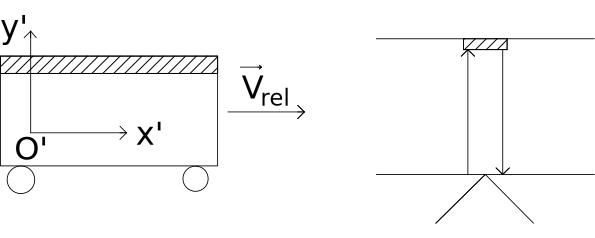
\includegraphics[width=15cm]{res/53reltempo}
        % \end{figure}
        \par Indichiamo con $\Delta\tau$ l'intervallo di tempo proprio misurato dall'osservatore proprio sul treno ($\Delta\tau=\frac{2d}{c}$). Analizziamo lo stesso fenomeno dal punto di vista dell'osservatore $O'$ fermo a terra.
        % \begin{figure}[h]
        %     \caption{Dettaglio del fenomeno visto da terra}
        %     \centering
        %     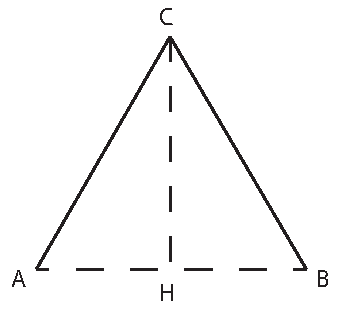
\includegraphics[width=15cm]{res/53reltempo2}
        % \end{figure}
        \begin{equation*}
            AC^2=AH^2+CH^2
        \end{equation*}
        \begin{equation*}
            (\frac{1}{2}c\cdot\Delta t)^2 = (\frac{1}{2}V_{rel}\Delta t)^2 + (\frac{1}{2}c\Delta\tau)^2
        \end{equation*}
        \begin{equation*}
            c^2\Delta{t}^2=V_{rel}^2\Delta{t} + c^2\Delta\tau2
        \end{equation*}
        \begin{equation*}
            \Delta{t}^2(c^2-V_{rel}^2) = \Delta{t}^2(1-\frac{V_{rel}^2}{c^2})
        \end{equation*}
        \begin{equation*}
            \Delta{t}=\Delta\tau\cdot\frac{1}{\sqrt{1-\frac{V_{rel}^2}{c^2}}}
        \end{equation*}
        \par Poniamo $\gamma=\frac{1}{\sqrt{1-\frac{V_{rel}^2}{c^2}}}$ e notiamo che $\gamma \geq 1 \forall V_{rel} \in R$. Otteniamo che
        \begin{equation}\label{eq:53reltempi}
            \Delta{t} = \gamma\Delta\tau
        \end{equation}
	\par $\gamma$ è il coefficiente di dilatazione relativistico.
    \subsection{Lunghezza propria e contrazione delle lunghezze}
	\par La lunghezza propria è quella misurata da un ossevatore fermo (o a riposo) rispetto all'oggetto.
	\par La misura di lunghezza effettuata da un osservatore in movimento rispetto ad un oggetto viene chiamata lunghezza non propria.
	Supponiamo che un osservatore $o'$ percorra la trave di un viadotto con velocità relativa $v_{rel}$. Indichiammo il suo viaggio sulla trave
	come il fenomeno. Per questo fenomeno l'ossevatore $o'$ misura un intervallo di tempo $\Delta\tau$, mentre un osservatore a terra misura
	un intervallo di tempo $\Delta t$.
	\par Dal punto di vista di $o$ $L_0=v_{rel}\cdot\Delta t$, per $o'$ $L=v_{rel}\cdot\Delta\tau$
	\par Dividendo membro a membro otteniamo $\frac{L}{L_0} = \frac{\Delta\tau}{\Delta t}$.
	\par $L=\frac{\Delta\tau}{\Delta t}\cdot L_0 = \frac{1}{\sigma}\cdot L_0$. Indichiamo con $\beta$ la quantità $\frac{v_{rel}}{c}$ e otteniamo
	che
	\begin{equation}L=\sqrt{1-\beta^2}\cdot L_0\end{equation}
	\par Questa equazione, conseguenza logica di $\Delta t = \gamma\Delta\tau$, viene chiamata contrazione delle lunghezze.
	\par Analizziamo una famosa verifica sperimentale dell'equazione della dilatazione dei tempi: quella della misura del tempo di dimezzamento
	di particelle subnucleari radioattive.
	\par Fu analizzato il decadimento di una particella subatomica chiamata muone ($\mu$). Tale particella è presente nei raggi cosmici oppure si
	può creare in laboratorio tramite opportune reazioni nucleari. È possibile misurare il tempo di decadimento di queste particelle sia in un 
	sistema di riferimento $o$ in cui sono ferme che in un sistema di riferimento che si muove a $0,99c$. Nel primo caso si bombarda un bersaglio di
	metallo pesante con protoni estremamente energetici ottenendo all'interno del bersaglio un grande numero di muoni carichi. Tali particelle,
	essendo radioattive, decadono emettendo altre particelle, che possono essere rilevate. Questa misura viene fatta da un osservatore $o$ a riposo.
	\par Per un osservatore $o'$ a riposo il tempo di dimezzamento ($T_\frac{1}{2}$) è di $1,77\cdot10^{-8}s=\Delta\tau$.
	\par La misura del tempo di dimezzamento può essere fatta generando i muoni per urti fra particelle ad altissima velocità, in modo tale che essi si
	muovano a $0,99c$ rispetto all'osservatore. La velocità di decadimento misurata è di $1,31\cdot10^{-7}s$, circa 7 volte maggiore rispetto
	all'osservatore fermo, in accordo con $\gamma$, che vale circa 7,1.
    \subsection{Trasformazioni di Lorentz}
	\subsubsection{Trasformazioni di Galileo}
	\begin{equation*}
	\begin{cases}
	x=x'+v_{rel}\cdot t'\\
	y=y'\\
	z=z'\\
	(t=t')
	\end{cases}
	\end{equation*}
	\subsubsection{Trasformazioni di Lorentz per la posizione}
	\begin{equation}
	\begin{cases}
	x=(x'+v_{rel}\cdot t')\cdot\gamma\\
	y=y'\\
	z=z'\\
	t=[t'+(\frac{v_{rel}}{c^2}x']\gamma
	\end{cases}
	\end{equation}

\tableofcontents
\end{document}